\documentclass[a4paper, 11pt]{article}
% ukazi za delo s slovenscino -- izberi kodiranje, ki ti ustreza
\usepackage[slovene]{babel}
\usepackage[utf8]{inputenc}
\usepackage[T1]{fontenc}
\usepackage[utf8]{inputenc}
\usepackage{amsmath,amssymb,amsfonts}
\usepackage{url}
\usepackage[normalem]{ulem}
\usepackage[dvipsnames,usenames]{color}
\usepackage{graphicx}
\usepackage{float}
\usepackage{verbatim}

% okolje za slike
\graphicspath{ {./slike/} }


% ukazi za matematicna okolja
%\theoremstyle{definition} % tekst napisan pokoncno
%\newtheorem{definicija}{Definicija}[section]
%\newtheorem{primer}[definicija]{Primer}
%\theoremstyle{remark}
%\newtheorem*{remark}{Opomba}


%\renewcommand\endprimer{\hfill$\diamondsuit$}


%\theoremstyle{plain} % tekst napisan posevno
%\newtheorem{lema}[definicija]{Lema}
%\newtheorem{izrek}[definicija]{Izrek}
%\newtheorem{trditev}[definicija]{Trditev}
%\newtheorem{posledica}[definicija]{Posledica}


% za stevilske mnozice uporabi naslednje simbole
\newcommand{\R}{\mathbb R}
\newcommand{\N}{\mathbb N}
\newcommand{\Z}{\mathbb Z}
\newcommand{\C}{\mathbb C}
\newcommand{\Q}{\mathbb Q}

% ukaz za slovarsko geslo
\newlength{\odstavek}
\setlength{\odstavek}{\parindent}
\newcommand{\geslo}[2]{\noindent\textbf{#1}\hspace*{3mm}\hangindent=\parindent\hangafter=1 #2}

% naslednje ukaze ustrezno popravi
\newcommand{\program}{Finančna matematika 1.~stopnja} % ime studijskega programa: Matematika/Finan"cna matematika
\newcommand{\imeavtorja}{Iza Čebulj, Barbara Pal} % ime avtorja
\newcommand{\naslovdela}{Najcenejše prirejanje v ravnini}
\newcommand{\letnica}{2022} 
\newcommand{\predmet}{Finančni praktikum}

% vstavi svoje definicije ...

%%%%%%%%%%%%%%%%%%%%%%%%%%%%%%%%%%%%%%%%%%%%%%%


\begin{document}

\thispagestyle{empty}
\begin{center}
\begin{minipage}{0.75\linewidth}
    \centering
    {\Large Univerza v Ljubljani \\ \program}
    \\
    \vspace{3cm}

    {\uppercase{\Large \textbf{\naslovdela}}} \\ \predmet\\
    \vspace{3cm}

    {\Large \imeavtorja\par}
    \vspace{9cm}

\end{minipage}
\end{center}

\noindent{\large
Ljubljana, \letnica}
\pagebreak

\thispagestyle{empty}
\tableofcontents
\listoffigures
\pagebreak

\section{Reševanje osnovnega problema najcenejšega prirejanja}
\subsection{Opis problema}
Množici $P$ z $2n$ točkami lahko priredimo neusmerjen graf $G(P,E),$ oziroma samo $G.$
Množica vozlišč grafa $G$ je kar množica $P,$ množica povezav v grafu $E$ pa so neurejeni pari vozlišč $(u,v),$ za katere velja $u,~v \in P$ in $u \neq v.$ 
Cena povezave je razdalja $d(u,v)$ med vozliščema $u$ in $v.$ \\
Popolno prirejanje na grafu $G$ oziroma v množici $P$ je taka množica povezav $M,$ za katero velja, da vsako vozlišče v $P$ sovpada z natanko eno povezavo v $M$.
Velikost popolnega prirejanja v množici velikosti $2n$ je $n.$ 
Ceno prirejanja definiramo kot $\sum_{(u,v) \in M} d(u,v),$ kar je vsota cen vseh povezav v $M.$ \\
Radi bi poiskali \emph{najcenejše popolno prirejanje} in njegovo ceno za različne $n.$

\subsection{Zapis problema kot celoštevilski linearni program}

\subsection{Programiranje rešitev in eksperimentiranje}
Pri svojem delu sva uporabljali spletno platformo \emph{CoCalc,} ki omogoča urejanje \emph{Jupyter} dokumentov.
Algoritem za iskanje najcenejšega prirejanja sva napisali v sistemu \emph{SageMath,} ki uporablja podobno sintakso kot \emph{Python.}
Najprej sva definirali funkcijo, ki nama je generirala $2n$ točk v enotskem kvadratu.

\begin{verbatim}
    def generiranje_tock_kvadrat(n):
    V = RDF^2 # vektorski prostor R^2 (ravnina)
    tocke = [V.random_element(min=0, max=1) for _ in range(2*n)]
    return tocke 
\end{verbatim}

Podobno sva definirali še funkciji, ki generirata točke v enotskem krogu in v enakostraničnem trikotniku.

Za tem pa sva želeli, da generirane točke predstavljajo vozlišča grafa, sam graf pa bo poln, torej so vse točke povezane med sabo
in tako lahko algoritem pri iskanju najkrajše razdalje oziroma najnižje cene upošteva vse možne razdalje oziroma cene.
V definicijo za generiranje grafa, kjer cene na povezavah predstavljajo razdaljo med točkami, sva torej vključili ukaze za $n,$ \emph{generiranje tock} in \emph{normo,}
s katerimi lahko izberemo število $2n$ točk, lik, iz katerega jih poberemo, ter normo, po kateri izračunamo razdaljo. 
Privzeta vrednost norme je $2,$ torej je to evklidska norma oziroma običajna razdalja med dvema točkama, seveda pa funkcija \texttt{graf} upošteva tudi normi $1$ in \emph{Infinity.}

\begin{verbatim}
    def graf(n, generiranje_tock, norma=2):
        tocke = generiranje_tock(n)
        G = graphs.CompleteGraph(len(tocke))
        for u, v in G.edges(labels=False):
            G.set_edge_label(u, v, (tocke[u] - tocke[v]).norm(norma))
        return G
\end{verbatim}

Definirali sva tudi funkcijo, ki graf izriše s približki cen povezav.
Tako izgleda generiran in izrisan graf na $6$ točkah, naključno izbranih v enotskem kvadratu, cene na povezavah pa so evklidske razdalje med vozlišči.
\begin{figure}[h!]
    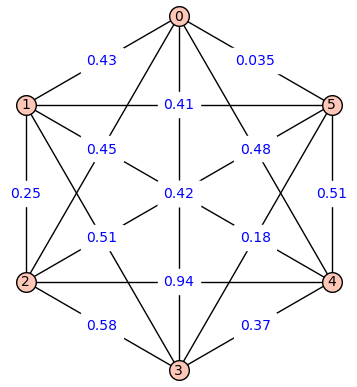
\includegraphics[scale=0.5]{graf1}
    \centering
\end{figure}

Končno pa sva s pomočjo \emph{SageMath-a} napisali še algoritem, ki s celoštevilskim linearnim programom
reši problem najcenejšega prirejanja, izpiše pare vozlišč, med katerimi so povezave v najcenejšem prirejanju $M,$ vsoto cen povezav v $M$ in nariše graf 
z označenimi povezavami, ki so v najcenejšem prirejanju.

\begin{verbatim}
def clp(G):
    p = MixedIntegerLinearProgram(maximization=False)
    b = p.new_variable(binary=True)
    p.set_objective(sum([w * b[Set(e)] for *e, w in G.edges(labels=True)]))

    for v in G:
        p.add_constraint(sum([b[Set(e)] 
                        for e in G.edges_incident(v, labels=False)]) == 1)

    cena = p.solve()
    b = p.get_values(b)

    M = [tuple(e) for e, i in b.items() if i]
    print(M) # pari vozlišč, med katerimi so povezave v najcenejšem prirejanju

    x = [w for *e, w in G.edges() if tuple(e) in M] # seznam cen povezav v M
    print(sum(x)) # vsota cen povezav v M

    H = Graph([(*e, N(w, digits=2)) for *e, w in G.edges(labels=True)])
    H.set_pos(G.get_pos())

    return H.plot(edge_colors={"red": M}, edge_labels=True) 
    # graf H z rdeče pobarvanimi povezavami iz prirejanja
\end{verbatim}

Ko na dobljenem grafu želimo najti povezave v najcenejšem prirejanju pa z uporabo funkcije \texttt{clp} dobimo
seznam parov vozlišč, med katerimi so povezave v najcenejšem prirejanju: \texttt{$[(0, 5), (1, 2), (3, 4)]$} in skupno vsoto cen teh povezav $0.6531541582221374$ (Slika \ref{fig:graf1clp}).

\begin{figure}[h!]
    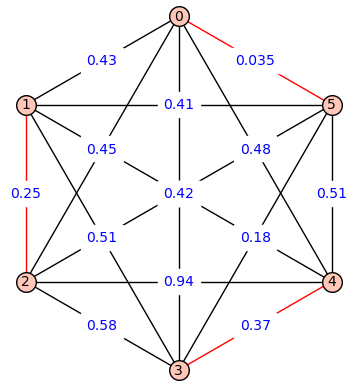
\includegraphics[scale=0.7]{graf1clp}
    \centering
    \caption{Graf z označenimi povezavami, ki so v najcenejšem prirejanju}
    \label{fig:graf1clp}
\end{figure}

\subsection{Analiza rezultatov}
Celoštevilski linearnih program sva večkrat pognali na različnih grafih, dobljene skupne vsote cen v najnižjem prirejanju pa sva izpisovali v \texttt{.csv} datoteko za lažji uvoz in obdelavo v programskem jeziku \emph{R.}

\subsubsection*{Časovna odvisnost algoritma}


\section{Dvobarvno najcenejše prirejanje}
\subsection{Opis problema}
Množico $P$ sestavljata množica $n$ rdečih točk, $R,$ in množica $n$ modrih točk $B,$ $P=R \cup B.$
V tem primeru je $G(P,E)$ dvodelen graf z lastnostjo, da med dvema točkama obstaja povezava, če in samo če sta različnih barv.
Cene povezav $(u,v)$ so tako kot v osnovnem primeru razdalje med vozlišči, $d(u,v).$
Spet iščemo najcenejše popolno prirejanje in njegovo ceno.

\subsection{Programiranje rešitev in eksperimentiranje}
Za programiranje rešitev sva ponovno uporabili \emph{SageMath.} Napisali sva funkcijo \texttt{dvobarven\underline{\space}graf,} ki je precej podobna prvotni funkciji,
prav tako pa sprejme ukaze za število točk, način generiranja točk oziroma lik in vrsto norme.

\begin{verbatim}
def dvobarven_graf(n, generiranje_tock, norma):
    G = graphs.CompleteBipartiteGraph(n, n)
    tocke = generiranje_tock(n)

    for u, v in G.edges(labels=False):
        G.set_edge_label(u, v, (tocke[u] - tocke[v]).norm(norma))
    return G
\end{verbatim}

Za iskanje najcenejšega prirejanja pa sva uporabili enak celoštevilski linearni program.

\begin{figure}[h!]
    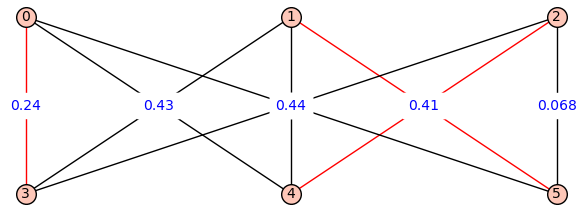
\includegraphics[scale=0.7]{dvobarvenclp}
    \centering
    \caption{Rešen problem najcenejšega prirejanja na dvobarvnem grafu, ko točke izberemo naključno v enakostraničnem trikotniku in za računanje razdalje med njimi uporabimo neskončno normo.}
    \label{fig:dvobarvenclp}
\end{figure}

\subsection{Analiza rezultatov}


\section{Zaključek}
% primerjava rezultatov obeh algoritmov

% \section{Literatura/Viri} ?

\end{document}